\section{Evaluations}
\label{sec:eval}

\setlength{\tabcolsep}{1pt}
\begin{table}[t]
\begin{CodeOut}
\begin{center}
\centering \caption {\label{tab:subjects} Subject applications and their characteristics.}
\begin {tabular} {|l|c|c|c|}
\hline
Application&\#Classes&\#Methods&\#Samples\\
\hline Java Util APIs&19&144&49858\\
\hline Java Transaction APIs&7&37&5555\\
\hline Java SQL APIs& 14 & 93 & 15052\\
\hline BCEL & 357 & 2691 & 9697\\
\hline HsqlDB& 143 & 1178 & 118610 \\
\hline Hibernate& 478 & 4334 & 105549 \\
\hline \textbf{Total}& 1018 & 8477 & 304321 \\
\hline
\end{tabular}\vspace*{-3ex}
\end{center}
\end{CodeOut}
\end{table}

We conducted two evaluations to assess the effectiveness of Alattin. Our empirical results show that there is a high percentage of \emph{balanced} and \emph{imbalanced} patterns in real applications. Our empirical results also show that Alattin effectively mines real rules from relevant code examples gathered through a CSE and is effective in detecting real defects. To show the significance of balanced and imbalanced patterns, we use the APIs provided by six open source libraries (three Java default API libraries and three popularly used open source libraries). For brevity, we refer to all subjects as applications. We also present our empirical evaluation for computing values for \emph{min\_sup} and \emph{alt\_sup} thresholds. The details of subjects and results of our evaluation are available at \texttt{https://sites.google.com/site/asergrp/ projects/alattin/}. We next present research questions addressed in our evaluation.
%-----------------------------------------------------------
\subsection{Research Questions}

In our evaluations, we address the following research questions.

\begin{itemize}
\item RQ1: How high percentage of balanced and imbalanced patterns exist in real applications? 
\item RQ2: How high percentage of false positives among detected violations are reduced by balanced and imbalanced patterns (while with no or low increase of false negatives)? As false positives are one of the common issues faced by existing static defect-detection techniques, this research question helps to show that more comprehensive patterns (such as balanced and imbalanced) help reduce the number of false positives. 
%\item RQ3: Do the violations detected by Alattin represent real defects?
\end{itemize}
%--------------------------------------------------------------------------
\subsection{Subject Applications}
\label{sec:subjects}

We next present subject applications used in our evaluations. In our evaluations, we used three Java default API libraries and three open source libraries. Table~\ref{tab:subjects} shows the characteristics of the subject applications. Columns ``Classes'' and ``Methods'' show the number of classes and methods, respectively. Column ``Samples'' shows the number of code examples gathered from a CSE for mining patterns. For example, Alattin gathered and analyzed $49,858$ code examples for the Java Util package.

The Java Util package includes the collections framework and other popular utilities used by many different applications. Java Transactions and Java SQL are industry standards for developing multi-tier server-side Java applications. The BCEL library, developed by Apache, is mainly used to analyze, create, and manipulate Java class files. Hibernate and HsqlDB abstract relational databases into an object-oriented methodology.\Comment{Columba is an open source email-client application written in Java. Columba provides a user-friendly graphical interface and is suitable for internationalization support.} We selected these applications because these applications are used as subjects in evaluating previous related approaches~\cite{WeimerN05, thummalapenta09:mining}.

%--------------------------------------------------------------------------
\subsection{RQ1: Balanced and Imbalanced Patterns}
\label{sec:balimbalpats}

\setlength{\tabcolsep}{1pt}
\begin{table*}[t]
\begin{SmallOut}
\begin{CodeOut}
\begin{center}
\centering \caption {\label{tab:minedpatterns} Patterns mined by Alattin}
\begin {tabular} {|l|c|c|c|c|c|c|c|c|}
\hline
Application&\#Total&\multicolumn{3}{|c|}{Categories of first 25 patterns}&\multicolumn{3}{|c|}{Subcategories of Real/Partial Rules}&Time\\
\cline{3-5}
\cline{6-8}
&Patterns&\#Real Rules&\#Partial Rules&\#False Positives&\#Single&\#Balanced&\#Imbalanced&(in min.)\\
\hline
\hline Java Util APIs&40&21&2&2&8&1&14& 9.75\\
\hline Java Transaction APIs&3&2&1&0&0&0&3& 1.67 \\
\hline Java SQL APIs&24&21&2&1&9&7&7& 2.64 \\
\hline BCEL&64&19&2&4&16&3&2& 12.02 \\
\hline HsqlDB&1&1&0&0&1&0&0& 18.06 \\
\hline Hibernate&12&11&0&1&10&1&0& 17.23 \\
\hline \textbf{Total}& 144 & 75 & 7 & 8 & 44 & 12 & 26 & 61.37 \\
\hline
\end{tabular}\vspace*{-5ex}
\end{center}
\end{CodeOut}
\end{SmallOut}
\end{table*}

We next address the first research question of whether balanced and imbalanced patterns often exist in real applications. To address this question, we configured Alattin, which by default accepts an application under analysis and mines patterns for third-party APIs, to accept a set of classes and methods directly. In this mode of operation, Alattin mines patterns (programming rules) for the APIs of the given classes and methods. For each subject application, we analyzed the top 25 patterns mined by Alattin. The results of our evaluation are shown in Table~\ref{tab:minedpatterns}.

Column ``Total Patterns'' shows the total number of patterns mined for each subject application. Column ``Categories of first 25 patterns'' shows the manual classification of the top 25 patterns into three categories: real rules, partial rules, and false positives among mined patterns. \emph{Real rules} describe properties that must be satisfied when using an API method. These real rules are of the form ``$P_1$ \textbf{or} $P_2$ \textbf{or} $\ldots$ \textbf{or} $P_i$ \textbf{or} $\hat{A_1}$ \textbf{or} $\hat{A_2}$ \textbf{or} $\ldots$ \textbf{or} $\hat{A_j}$'', where all alternatives (both frequent and infrequent) represent real properties. In contrast to real rules, \emph{partial rules} are of the form ``$P_1$ \textbf{or} $P_2$ \textbf{or} $\ldots$ \textbf{or} $P_i$ \textbf{or} $\hat{A_1}$ \textbf{or} $\hat{A_2}$ \textbf{or} $\ldots$ \textbf{or} $\hat{A_j}$'', where all frequent alternatives such as $P_1$, $P_2$, ..., $P_i$ represent real properties and some of the infrequent alternatives such as $\hat{A_1}$ and $\hat{A_2}$ do not represent real properties. The reason for introducing partial rules is that partial rules are as effective as real rules in reducing false-positive defects; however, partial rules can increase false-negative defects due to false-positive infrequent alternatives (among mined patterns) such as $\hat{A_1}$ and $\hat{A_2}$. We used available on-line documentations, JML specifications\footnote{\texttt{http://www.eecs.ucf.edu/~leavens/JML/}}, or source code of applications for classifying mined patterns into these three categories. 

Our results show that Alattin can mine a high percentage of patterns (ranging from 84\% to 100\%) that represent real or partial rules. These results show that Alattin can effectively mine real programming rules that can be used for tasks such as program comprehension and defect detection. To show that balanced and imbalanced patterns often exist, we further classified real and partial rules into three subcategories: balanced, imbalanced, and single patterns. The definitions of these subcategories are described in Section~\ref{sec:probdef}. Column ``Subcategories of Rules/Partial Rules'' shows the results of our further classification. Figure~\ref{fig:balimbal} shows the distribution chart for balanced, imbalanced, and single patterns. In the distribution chart, x-axis shows subject applications and y-axis shows the percentages of Rules/Partial rules classified into three subcategories. 

\begin{figure}[t]
\centering
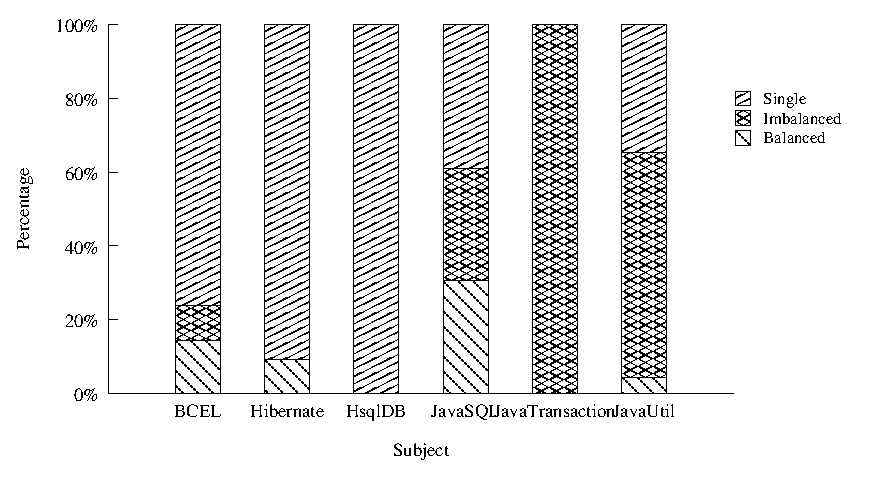
\includegraphics[scale=0.60,clip]{figs/Alattin_Patterns.eps}\vspace*{-1ex}
\caption{\label{fig:balimbal}Classification of Real/Partial Rules into Balanced, Imbalanced, and Single patterns}\vspace*{-5ex}
\end{figure}

Our results show that imbalanced patterns range from 30\% to 100\% (on average 65\%) among the Java default API libraries, whereas these patterns range from 0\% to 9.5\% (on average 5\%) among the patterns of libraries BCEL, Hibernate, and HsqlDB. The difference in results between Java default libraries and other open source libraries with respect to imbalanced patterns could be that Java default API libraries provide different ways of writing code for achieving the same programming task, whereas other open source libraries such as BCEL or Hibernate often provide a single way for writing code. Furthermore, balanced patterns range from 0\% to 30\% (on average 9.69\%) among all six subject applications. In summary, our results show that both a high percentage of balanced and imbalanced patterns exist among real applications. 

We next present example balanced and imbalanced patterns mined by Alattin in Figure~\ref{fig:balimbalpar}. For each pattern, we show the method name, all alternatives, and their support values (denoted by $SUP$ for frequent alternatives and $ABS$ for infrequent alternatives). We show the $SUP$ value for frequent alternatives and both $SUP$ and $ABS$ values for infrequent alternatives. The balanced pattern shown in Figure~\ref{fig:balimbalpar}A describes that there should be either a constant check such as greater than zero after the \CodeIn{read} method ($P_1$) or a \CodeIn{null-check} on the return of \CodeIn{getNextEntry} before the \CodeIn{read} method ($P_2$). Both alternative patterns are frequent as their support values are greater than the \emph{min\_sup} value. The imbalanced pattern shown in Figure~\ref{fig:balimbalpar}B 
describes three different ways of using the \CodeIn{getString} method of the \CodeIn{java.sql.ResultSet} class. Among the alternatives of the pattern, $P_1$ is the only frequent alternative, whereas all the other alternatives are infrequent. The \CodeIn{ResultSet.getString} method throws \CodeIn{SQLException} if the input column index is more than the number of columns in the database. The mined pattern presents different ways of ensuring that the index value is between zero and the number of columns. In this imbalanced pattern, the $SUP$ value of $P_2$ alternative is 0.01, which is lower than $min\_sup$. This pattern is chosen as infrequent alternative since its $ABS$ value is 0.28, which is higher than the $alt\_sup$ value. 

\begin{figure}[t]
\textbf{\emph{A}}. \textbf{Balanced pattern}\\
Method: \CodeIn{ZipInputStream.read (byte[], int, int)}\\
Pattern: ``$P_1$ \textbf{or} $P_2$''\\
$P_1$:``\CodeIn{const-check} on the return of \CodeIn{ZipInputStream. \hspace*{0.2in}read} with 0''(SUP($P_1$): 0.79)\\
$P_2$:``\CodeIn{null-check} on the return of \CodeIn{ZipInputStream. \hspace*{0.2in}getNextEntry} before
\CodeIn{ZipInputStream.read}''\\ (SUP($P_2$): 0.55)\\
\\
\textbf{\emph{B}}.\textbf{Imbalanced pattern}\\
Method: \CodeIn{ResultSet.getString (int)}\\
Pattern: ``$P_1$ \textbf{or} $\hat{P_2}$ \textbf{or} $\hat{P_3}$''\\
$P_1$:``\CodeIn{boolean-check} on the return of \CodeIn{ResultSet.next} \hspace*{0.2in}before  \CodeIn{ResultSet.getString}'' (SUP($P_1$): 0.88) \\
$P_2$:``\CodeIn{boolean-check} on the return of \CodeIn{ResultSet.first} \hspace*{0.2in}before \CodeIn{ResultSet.getString}'' \\
\hspace*{0.4in} (ABS($P_2$): 0.28, SUP($P_2$): 0.01) \\
$P_3$:``\CodeIn{null-check} on return of \CodeIn{ResultSet.getString}'' \\
\hspace*{0.4in} (ABS($P_3$): 0.4, SUP($P_3$): 0.08) \\
\Caption{\label{fig:balimbalpar} Balanced and imbalanced patterns}
\end{figure}

Column ``Time'' presents the amount of time taken (in minutes) by Alattin for analyzing gathered code examples and mining patterns. The amount of processing time depends on the number of code examples gathered for an application under analysis. For example, Alattin took $9.75$ minutes for mining patterns from $49,858$ code examples gathered for the Java Util package. All experiments were conducted on a machine with 3.0GHz Xeon processor and 4GB RAM.

%--------------------------------------------------------------------------
\subsection{RQ2: False Positives and False Negatives}
\label{sec:defopensource}

We next address the second research question of whether balanced and imbalanced patterns help reduce a high percentage of false positives among detected violations. We also address whether these patterns introduce \emph{only} no or a low percentage of false negatives among detected violations. To address this question, we applied mined patterns on gathered code examples themselves in three different modes. In each mode, we compute a Programming Rules Set, say $PRS$, from the patterns of single, balanced, and imbalanced categories in different ways and apply each programming rule individually for detecting violations. We use notations ``$P_1$'', ``$P_1$ \textbf{or} $\ldots$ \textbf{or} $P_i$'', ``$P_1$ \textbf{or} $\ldots$ \textbf{or} $P_i$ \textbf{or} $\hat{A_1}$ \textbf{or} $\ldots$ \textbf{or} $\hat{A_j}$'' for single, balanced, and imbalanced patterns, respectively.

\textbf{Existing Mode (EM).} EM reflects the methodology adopted by existing approaches~\cite{Engler2001deviant,Zhenmin2005PRMiner,acharya06:mining} for detecting violations. This mode serves as a baseline to show the benefits of balanced and imbalanced patterns. For a single-category pattern, we add to $PRS$ the corresponding rule for each alternative $P_1$ of the mined pattern. For a balanced-category pattern, we first split the alternatives into individual patterns and add them to $PRS$. We add to $PRS$ $i$ corresponding rules for the balanced pattern ``$P_1$ \textbf{or} $\ldots$ \textbf{or} $P_i$'' with $i$ alternatives. For an imbalanced-category pattern, we discard infrequent alternatives and split frequent alternatives. Similar to the way of handling a balanced pattern, we add to $PRS$ $i$ corresponding rules for the imbalanced pattern ``$P_1$ \textbf{or} $\ldots$ \textbf{or} $P_i$ \textbf{or} $\hat{A_1}$ \textbf{or} $\ldots$ \textbf{or} $\hat{A_j}$'' with $i$ frequent alternatives.

\textbf{Balanced Mode (BM).} BM helps show the benefits of balanced patterns in reducing false positives among detected violations. For a single- or balanced-category pattern, we add to $PRS$ one corresponding rule for each mined pattern. For an imbalanced-category pattern, we discard infrequent alternatives in the pattern. Discarding infrequent alternatives of an imbalanced pattern transforms the pattern into a balanced pattern. We add to $PRS$ one corresponding rule for each such transformed pattern.

\textbf{(Im)balanced Mode (IM).} IM helps show the benefits of imbalanced patterns. We add to $PRS$ one corresponding rule for each mined pattern of all categories.
 
\setlength{\tabcolsep}{1pt}
\begin{table*}[t]
\begin{SmallOut}
\begin{CodeOut}
\begin{center}
\centering \caption {\label{tab:detectedviolations} Violations detected by Alattin in Open Source Applications}
\begin {tabular} {|l|c|c|c|c|c|c|c|c|c|c|c|}
\hline
Application&Total&\multicolumn{2}{|c|}{Existing Mode (EM)}&\multicolumn{4}{|c|}{Balanced Mode (BM)}&\multicolumn{4}{|c|}{(Im)balanced Mode (IM)}\\
\cline{3-12}
&&Defects&FP&Defects&FN&FP&\% Reduction in FP&Defects&FN&FP&\% Reduction in FP\\
&&&&&&& from EM mode&&&& from EM Mode\\
\hline
\hline Java Util APIs& 974 & 37 & 104 & 37 & 0 & 104 & 0 & 36 & 1 & 74 & 28.85\\
\hline Java Transaction APIs& 156 & 51 & 105 & 51 & 0 & 105 & 0 & 47 & 4 & 76 & 27.62\\
\hline Java SQL APIs& 315 & 56 & 143 & 56 & 0 & 90 & 37.06 & 53 & 3 & 81 & 43.36\\
\hline BCEL& 160 & 2 & 14 & 2 & 0 & 8 & 42.86 & 2 & 0 & 6 & 57.14\\
\hline HsqlDB& 1 & 1 & 0 & 1 & 0 & 0 & 0 & 1 & 0 & 0 & 0\\
\hline Hibernate& 22 & 10 & 9 & 10 & 0 & 8 & 11.11 & 10 & 0 & 8 & 11.11\\
\hline
\hline \textbf{Average} & & & & & & & \textbf{15.17} & & & & \textbf{28.01}\\ 
\hline
\end{tabular}\vspace*{-3ex}
\end{center}
\end{CodeOut}
\end{SmallOut}
\end{table*}

Table~\ref{tab:detectedviolations} shows violations detected in each mode for all applications. Column ``Total'' shows the total number of violations. Given the large number of detected violations in subjects such as the Java Util package, we present the violations detected by the top 10 patterns (shown in Columns EM, BM, and IM). Our results show that there is a reduction in the number of false positives by 15.17\% in BM and 28.01\% in IM. In summary, the results show that balanced and imbalanced patterns help effectively reduce the number of false positives among detected violations. Our results also show that the number of false negatives introduced in Balanced and (Im)balanced modes is quite minimal. These false negatives occur due to the partial rules shown in Table~\ref{tab:minedpatterns}. 

To further show the effectiveness of our approach, we computed a metric called \emph{accuracy}~\cite{tan06:data} that is based on four different factors: true positives (TP), false positives (FP), false negatives (FN), and true negatives (TN). In each mode, we consider the number of detected defects and the number of false positives as TP and FP, respectively. As EM is our baseline, we assume the number of FN and TN as zero. For mode BM, we compute false negatives as \CodeIn{Number of defects in mode EM - Number of defects in mode BM}. These false negatives show the number of defects missed in mode BM compared to mode EM due to partial rules mined by our approach. Similarly, we compute true negatives as \CodeIn{Number of false positives in mode EM - Number of false positives in mode BM}. These true negatives show the number of false positives reduced in mode BM compared to mode EM due to balanced and imbalanced patterns. We use the same way for computing these four factors for mode IM. We next compute the accuracy metric from these four factors using the formula shown below:

\begin{CodeOut}
\hspace*{0.7in}Accuracy = $\frac{TP + TN}{TP + FP + FN + TN}$
\end{CodeOut}
\newline

The rationale behind our accuracy metric is that higher accuracy metric values are assigned to those modes that reduce a higher number of both false positives and false negatives. Therefore, if our balanced and imbalanced patterns increase false negatives or do not decrease false positives, the corresponding accuracy metric values are also low. Figure~\ref{fig:accuracy} shows the computed accuracies for modes EM, BM, and IM. The figure shows that mode IM has higher accuracy metric values compared to modes EM and BM. Our results indicate that our balanced and imbalanced patterns help reduce false positives with \emph{only} a minimal increase in false negatives.

\begin{figure}[t]
\begin{CodeOut}
\begin{alltt}
00:public describeProcedureCall() throws 
\hspace*{1.5in}SQLException \{
01:\hspace*{0.2in}PreparedStatement ps = null; ...
02:\hspace*{0.2in}ResultSet rs = ps.executeQuery();
03:\hspace*{0.2in}if(!rs.first())  \{
04:\hspace*{0.4in}...
05:\hspace*{0.4in}return;
06:\hspace*{0.2in}\}
07:\hspace*{0.2in}...
08:\hspace*{0.2in}do \{
09:\hspace*{0.4in}String datatype = rs.getString(2);
10:\hspace*{0.4in}...
11:\hspace*{0.2in}\} while(rs.next()); ...
12:\}
\end{alltt}
\end{CodeOut}\vspace*{-1ex}
\Caption{\label{fig:buggycode} A code example gathered from the Debian tools source code.}\vspace*{-3ex}
\end{figure}

We next present an example to show how imbalanced patterns help reduce the number of false positives.  Figure~\ref{fig:buggycode} shows a code example of class \CodeIn{com.sap.dbtech.jdbc.Parseinfo} collected from the SVN repository of the Debian\footnote{\texttt{http://www.debian.org/}} tools. For simplicity, irrelevant code portions are omitted from the code example. The frequent alternative $P_1$ of the imbalanced pattern shown in Figure~\ref{fig:balimbalpar}B describes that there should be a \CodeIn{boolean} check on the return of \CodeIn{ResultSet.next} before \CodeIn{ResultSet.getString}. With just the $P_1$ alternative, an existing mining approach detects a violation in this code example since the code example does not include a \CodeIn{boolean} check on the return of \CodeIn{ResultSet.next} preceding the first invocation of \CodeIn{ResultSet.getString}. However, the code example does not have a defect in using the \CodeIn{getString} method since the \CodeIn{if} condition in Statement 3 ensures that there is at least one element in \CodeIn{ResultSet} before reaching  Statement 9. This code example illustrates the use of imbalanced patterns in reducing false positives among detected violations.

\begin{figure}[t]
\centering
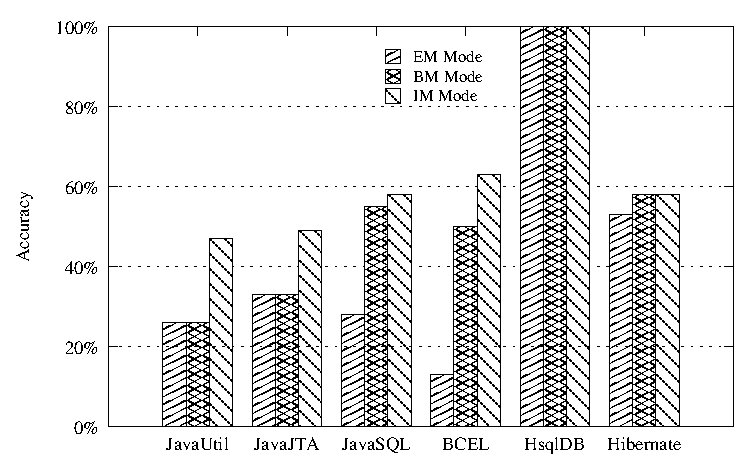
\includegraphics[scale=0.70,clip]{figs/Alattin_Accuracy.eps}\vspace*{-1ex}
\caption{Accuracy metric values for Modes EM, BM, and IM.} \label{fig:accuracy}\vspace*{-4ex}
\end{figure}

\Comment{TODO:
Although there is a significant reduction in the number of false positives in Mode 3, false positives still exist in Mode 3. These false positives are primarily due to two major reasons. First, implementation limitations of our current prototype. We plan to address these limitations in our future work. Second, limitations due to conservative nature of static analysis.} 
%-----------------------------------------------------------------------------------------
\Comment{
\subsection{RQ3: Real Defects}
\label{sec:columba}

We next address the third research question of whether the detected violations of Alattin represent real defects.
To address this question, we applied our Alattin on the Columba application.
The reason for selecting Columba is that this application is used as a subject in evaluating a previous related approach~\cite{wasylkowski07:detecting}. The Columba application includes $1,165$ classes and $6,894$ 
methods that contain a total of $91,508$ lines of Java code. 
We used Alattin to mine patterns of APIs used by Columba 
and detected violations using those mined patterns.
Alattin identified that Columba reuses $541$ third-party classes and $2,225$ third-party methods,
and mined patterns for those third-party methods by interacting with a CSE. 
Alattin gathered and analyzed $309,757$ code examples ($\approx$ 50 million LOC)
for mining these patterns. 

Alattin mined a total of $195$ patterns related to the third-party methods 
used by Columba. These $195$ mined patterns detected a total of $478$ violations
in Mode 3 that considers all three categories of mined patterns. 
We manually analyzed all $29$ violations detected with the top $25$ mined patterns.
We classified $29$ violations into two violation categories: defects
and false positives. The defect category indicates a real defect in the application
under analysis, whereas a false positive indicates that detected violation is not a
real defect. 

\setlength{\tabcolsep}{1pt}
\begin{table}[t]
\begin{SmallOut}
\begin{CodeOut}
\begin{center}
\centering \caption {\label{tab:columba} Evaluation results with Columba.}
\begin {tabular} {|c|c|l|l|c|c|}
\hline
Pattern&Support&Pattern&Pattern&\multicolumn{2}{|c|}{Categories of violations}\\
\cline{5-6}
Rank&&category&sub-category&\#Defect&\#FP\\
\hline
\hline 1&1&Rule& Balanced & &\\
\hline 2&1&Rule& Balanced & 2 &\\
\hline 3&1&FP& & &\\
\hline 4&1&FP& & & 1 \\
\hline 5&1&Rule& Single & 1 & \\
\hline 6&0.93&Rule& Imbalanced & &\\
\hline 7&0.92&Rule& Imbalanced & 1 &\\
\hline 8&0.91&Rule& Imbalanced & 7 & 6\\
\hline 9&0.89&Rule& Single & &\\
\hline 10&0.88&Rule& Single & &\\
\hline 11&0.88&Rule& Single & & 3\\
\hline 12&0.87&Rule& Imbalanced & &\\
\hline 13&0.86&Rule& Imbalanced & &\\
\hline 14&0.82&Rule& Balanced & &\\
\hline 15&0.81&Rule& Single & &\\
\hline 16&0.80&Rule& Single & 1 & 2\\
\hline 17&0.79&Rule& Imbalanced & 2 &\\
\hline 18&0.79&Rule& Single & &\\
\hline 19&0.77&Rule& Single & &\\
\hline 20&0.76&Rule& Imbalanced & & 1\\
\hline 21&0.75&Rule& Balanced & &\\
\hline 22&0.75&Rule& Single & &\\
\hline 23&0.75&Rule& Imbalanced & 2 &\\
\hline 24&0.73&Rule& Single & &\\
\hline 25&0.73&Rule& Single & &\\
\hline
\end{tabular}
\end{center}
\end{CodeOut}
\end{SmallOut}
\end{table}

Table~\ref{tab:columba} shows our evaluation results. For each mined pattern in the top 25, the table shows support and pattern category (rule, partial rule or false positive) in Columns ``Support'' and ``Pattern category'', respectively. Column ``Pattern sub-category'' shows further classification of rules into balanced, imbalanced, and single patterns. Our results show that $23$ mined patterns of the top $25$ are real rules. Among these $23$ mined patterns, there are $4$ balanced, $8$ imbalanced, and $11$ single patterns. Furthermore, there are no partial rules among these mined patterns.
Therefore, our approach does not produce any false negatives among detected violations in Columba.

Among $29$ violations, $16$ violations are real defects in the Columba application and $13$ violations are false positives.
In our analysis, we found that $12$ false positives are primarily due to our implementation limitations such as intra-procedural analysis or lack of path-sensitive analysis. We plan to address these implementation limitations in near future work and these limitations can be addressed without much difficulty. The remaining one false positive is due to a false-positive pattern mined by our approach. We next describe the false-positive pattern shown in Rank 4 of Table~\ref{tab:columba}. The mined pattern is ``\CodeIn{null-check} on \CodeIn{return} after \CodeIn{JList.getSelectedValue} before \CodeIn{JCheckBox}.\\\CodeIn{removeActionListener}''. Although this pattern is found in all code examples using the \CodeIn{JCheckBox.removeActionListener}, we did not find the pattern in related Java documentation. Therefore, we classified the pattern as a false-positive pattern.

We next describe defects detected by Alattin in Columba. We confirmed these defects through inspecting the source code of associated class. Alattin detected a defect in the \CodeIn{removeDoubleEntries} method of the \CodeIn{MessageBuilderHelper} class. We show the code sample of that method as below:\vspace{-1ex}

\begin{CodeOut}
\begin{alltt}
private static String removeDoubleEntries(String input) \{
\hspace*{0.1in}Pattern sP = Pattern.compile("s*(<[^s<>]+>)s*");
\hspace*{0.1in}ArrayList entries = new ArrayList();
\hspace*{0.1in}Matcher matcher = sP.matcher(input);
\hspace*{0.1in}while (matcher.find()) \{
\hspace*{0.3in}entries.add(matcher.group(1));	\}
\hspace*{0.1in}Iterator it = entries.iterator(); ...
\hspace*{0.1in}String last = (String) it.next(); ... \}
\end{alltt}
\end{CodeOut}\vspace{-1ex}

The method \CodeIn{removeDoubleEntries} tries to identify character sequences
that match with a regular expression. If the given input string does not match with the regular expression
``\CodeIn{s*(<[\^s<>]+>)s*}'', no elements will be added to the \CodeIn{entries} list.
The preceding code sample violated the mined rule ``\CodeIn{boolean-check} on \CodeIn{return} of
\CodeIn{Iterator.hasNext} \CodeIn{before} \CodeIn{Iterator.next}'',
which describes that \CodeIn{hasNext} must be invoked before 
calling \CodeIn{next} of the \CodeIn{Iterator} class.  In the code sample,
the first element from the \CodeIn{it} variable is retrieved without checking whether there
are any elements in the list through \CodeIn{hasNext}. Moreover, 
the retrieved variable is type-casted to a string. This defect
can cause \CodeIn{NoSuchElementException} in the described scenario. Although the current method
is \CodeIn{private}, the public caller methods of the current class do not handle any
exceptions, resulting in the propagation of the exception to their call sites. 

Another detected defect is related to the JPIM\footnote{\texttt{http://jpim.cvs.sourceforge.net/jpim/}} 
library used by Columba. Columba invokes the method \CodeIn{unmarshallContacts}
of the class \CodeIn{ContactUnmarshaller} that is defined by the JPIM library. 
Alattin identified the pattern ``\CodeIn{null-check} on \CodeIn{return after} 
\CodeIn{ContactUnmarshaller.unmarshallContacts}'', which indicates that a \CodeIn{null} check must be 
performed on the return value of the \CodeIn{unmarshallContacts} method. 
As this pattern is not available in the documentation, we confirmed this pattern by inspecting 
source code of the JPIM library.
In Columba, this method is invoked in the class \CodeIn{VCardParser}
and no \CodeIn{null} check on the return variable was done. The absence of the \CodeIn{null} check 
can cause a \CodeIn{NullPointerException}.

\Comment{Another defect is detected in the method \CodeIn{readInByteArray}
of the class \CodeIn{StreamUtils}. We show the code example of the \CodeIn{readInByteArray} method as below:\vspace{-2ex}

\begin{CodeOut}
\begin{alltt}
...
byte[] result = new byte[in.available()];
in.read(result);
in.close();
return result;
\end{alltt}
\end{CodeOut}\vspace{-2ex}

The preceding code example violated the mined pattern ``\CodeIn{const-check} on
\CodeIn{return} of \CodeIn{InputStream.read}'', which describes that the return value of the \CodeIn{read}
function must be verified. This return value gives the number of bytes that are actually read
from the input stream. }}
%--------------------------------------------------------------------------

\begin{figure*}[t]
\centering
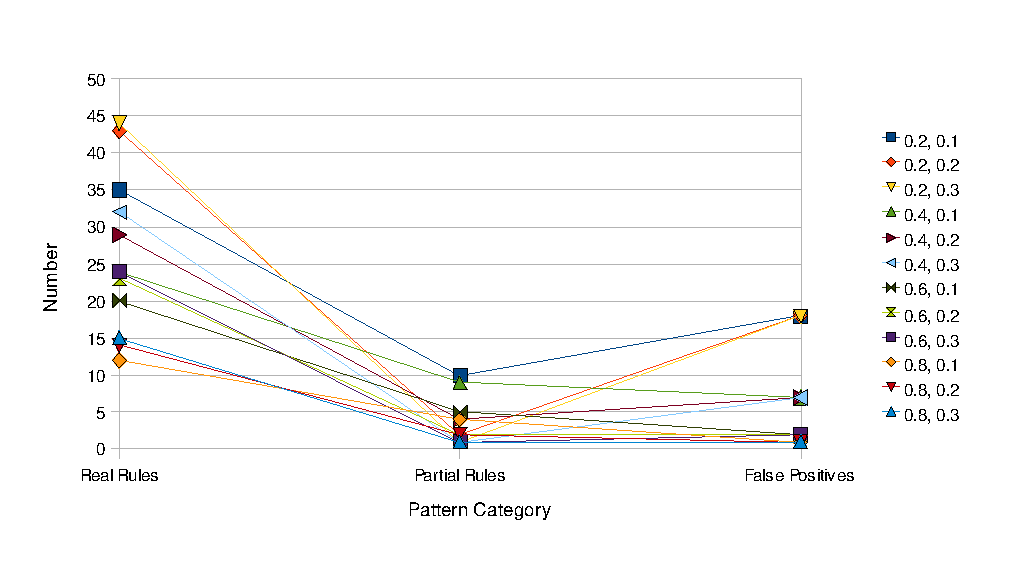
\includegraphics[scale=0.80,clip]{figs/Threshold_Categories.eps}
\caption{Distribution of rules, partial rules, and false positives.} \label{fig:thresholdminsup}\vspace*{-2ex}
\end{figure*}
%--------------------------------------------------------------------------
\Comment{\subsection{Summary of the Evaluation}
\label{sec:evalsummary}

The major advantage of Alattin compared to existing approaches ~\cite{Zhenmin2005PRMiner,acharya06:mining,chang07:finding,acharya07:mining,wasylkowski07:detecting} is that Alattin can identify real rules due to the large number of data points used for mining the programming rules. The number of false positive patterns mined by Alattin is relatively low compared to other existing approaches as shown in our first evaluation. Alattin confirmed three out of four defects that are reported in the literature and are related to neglected conditions. Alattin detected three new defects in the Columba application, which is a popular email client. We showed that Alattin can identify defects in existing open source applications when a set of interested APIs is given as input. This feature could be quite useful for APIs such as security APIs. We also showed that Alattin can deal with
the scalability issues in processing the large number of related code examples gathered from a CSE.}

%-----------------------------------------------------------------------------
\subsection{Threshold Values}
\label{sec:thresholds}

We conducted an empirical study with the Java Util package for computing values for \emph{min\_sup} and \emph{alt\_sup} thresholds. The \emph{min\_sup} threshold affects the number of real rules and false positives among mined patterns. For example, choosing a high value for the \emph{min\_sup} threshold leads to a low number of false positives but also leads to a low number of real rules among mined patterns. In contrast, the \emph{alt\_sup} threshold affects the number of imbalanced patterns among mined patterns. For example, choosing a low value for \emph{alt\_sup} increases the number of imbalanced patterns among mined patterns and also increases the number of partial rules that can result in false negatives among detected violations.

To compute values for \emph{min\_sup} and \emph{alt\_sup} with reasonable tradeoffs, we applied our approach on the Java Util package with various values for these two thresholds. We classified mined patterns for each combination of \emph{min\_sup} and \emph{alt\_sup} values into real rules, partial rules, and false positives. We further classified the real and partial rules into balanced and imbalanced patterns. Figures~\ref{fig:thresholdminsup} and~\ref{fig:thresholdaltsup} show the results of our evaluation. For our evaluations, we used \emph{min\_sup} as 0.4 and \emph{alt\_sup} as 0.2 since these two thresholds have reasonable tradeoffs.

\begin{figure*}[t]
\centering
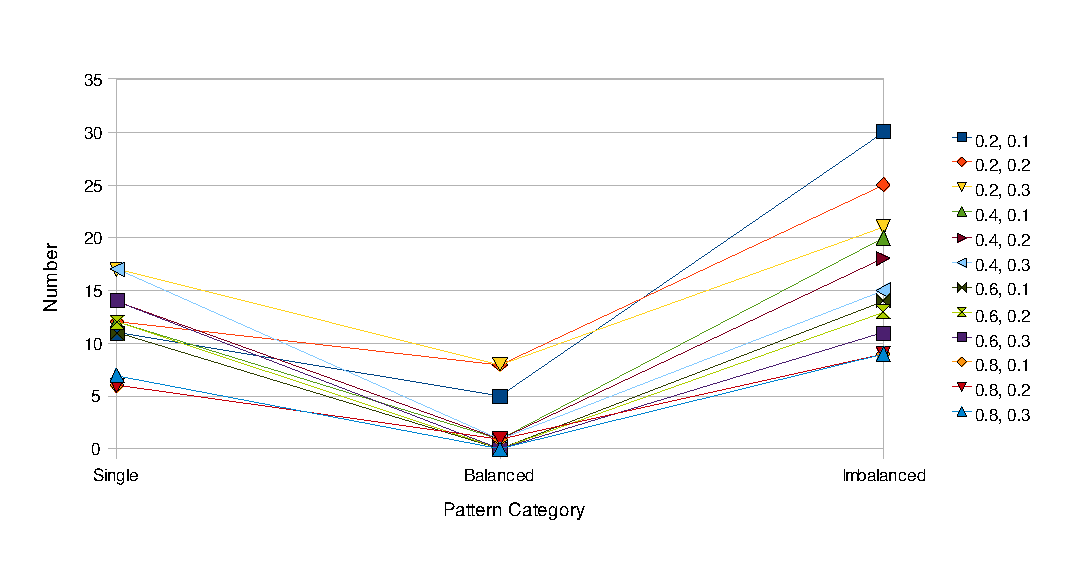
\includegraphics[scale=0.80,clip]{figs/Threshold_subcategories.eps}
\caption{Distribution of single, balanced, and imbalanced patterns.} \label{fig:thresholdaltsup}
\end{figure*}